\documentclass[12pt,a4paper]{article}

% ── Core packages ──────────────────────────────────────────────────────────────
\usepackage{amsmath}
\usepackage{amssymb}
\usepackage{geometry}
\geometry{margin=2.5cm}
\usepackage{booktabs}
\usepackage{xcolor}
\usepackage{hyperref}
\usepackage{listings}
\usepackage{pgfplots}
\pgfplotsset{compat=1.18}
\usepackage{tcolorbox}
\tcbuselibrary{skins, breakable}
\usepackage{enumitem}
\usepackage{fancyhdr}
\usepackage{tikz}
\usepackage{array}

% ── tcolorbox environments ─────────────────────────────────────────────────────
\newtcolorbox{curiositybox}[1]{colback=yellow!10, colframe=orange!80!black, fonttitle=\bfseries, title=#1, breakable}
\newtcolorbox{infobox}[1]{colback=blue!5, colframe=blue!60!black, fonttitle=\bfseries, title=#1, breakable}
\newtcolorbox{mistakebox}[1]{colback=red!5, colframe=red!60!black, fonttitle=\bfseries, title=#1, breakable}
\newtcolorbox{learnbox}[1]{colback=green!5, colframe=green!60!black, fonttitle=\bfseries, title=#1, breakable}

% ── lstlisting (Python) ────────────────────────────────────────────────────────
\lstset{language=Python, basicstyle=\ttfamily\small, keywordstyle=\color{blue},
        commentstyle=\color{gray}, stringstyle=\color{orange},
        showstringspaces=false, numbers=left, numberstyle=\tiny,
        breaklines=true, frame=single}

% ── fancyhdr ───────────────────────────────────────────────────────────────────
\pagestyle{fancy}
\fancyhf{}
\lhead{Topic 03: Inverse Laplace Transform}
\rhead{Unit IV --- Laplace Transforms}
\cfoot{\thepage}

% ── Title ──────────────────────────────────────────────────────────────────────
\title{Topic 03: Inverse Laplace Transform \\ \large Unit IV --- Laplace Transforms}
\author{23A54201 --- Mathematics IV (Transform Techniques) \\
        JNTUA College of Engineering (Autonomous)}
\date{}

% ══════════════════════════════════════════════════════════════════════════════
\begin{document}
\maketitle
\tableofcontents
\newpage

% ══════════════════════════════════════════════════════════════════════════════
\section{Opening Hook}

\begin{curiositybox}{Hook}
You solved an ODE using the Laplace Transform and arrived at a beautiful, tidy algebraic
expression: $Y(s) = \dfrac{3s+5}{(s-1)(s+2)}$. Wonderful --- except your actual answer
needs to be in terms of $t$, not $s$! This is the return journey. Just like a translator
who converts a message back to your native language, the inverse Laplace transform brings
your solution home to the time domain.
\end{curiositybox}

% ══════════════════════════════════════════════════════════════════════════════
\section{Why This Topic Exists}

``Before we begin, here is the honest answer to why you are reading this\ldots''

Every time you apply the Laplace transform to solve an ODE, you obtain a neat
algebraic expression $Y(s)$ in the frequency domain.  That expression is not
your final answer --- your answer is the function $y(t)$ that satisfies the
original equation.  The inverse Laplace transform is the \emph{only} systematic
tool for making that final conversion.  Without it, all the machinery of Laplace
methods is incomplete.

\medskip
\noindent The table below shows what happens when students skip key steps in the
inversion process.

\begin{center}
\begin{tabular}{@{} p{6cm} p{7cm} @{}}
\toprule
\textbf{What students skip} & \textbf{Consequence} \\
\midrule
Stopping the solution at $Y(s)$ &
    Never actually answering what the ODE asked for ($y(t)$) \\
\midrule
Skipping partial fractions setup &
    Being unable to match $F(s)$ to any table entry \\
\midrule
Forgetting to complete the square for quadratics &
    Missing shifted sine/cosine forms entirely \\
\bottomrule
\end{tabular}
\end{center}

\begin{learnbox}{Key Takeaway}
The inverse Laplace transform is not optional --- it is the essential final step
that converts an algebraic $s$-domain answer back to the $t$-domain solution your
problem actually asked for.
\end{learnbox}

% ══════════════════════════════════════════════════════════════════════════════
\section{You Already Know This (Intuition First)}

Think of the standard Laplace transform table as a phrasebook for two languages:
the time-domain language ($f(t)$, $g(t)$, \ldots) and the $s$-domain language
($F(s)$, $G(s)$, \ldots).  When you compute a forward transform you read the
phrasebook left-to-right.  When you compute an inverse transform you read it
\emph{right-to-left}.  The words and grammar are the same; only the direction
of reading changes.

The skill, then, is simply \emph{pattern recognition on the $F(s)$ side} ---
spotting that $\dfrac{1}{s+3}$ looks like $\dfrac{1}{s-a}$ with $a=-3$, so
the inverse must be $e^{-3t}$.  You already possess this skill from Topic 01
and 02; you are just applying it in reverse.

% ══════════════════════════════════════════════════════════════════════════════
\section{Definition of the Inverse Transform}

\begin{infobox}{Inverse Laplace Transform --- Definition}
If $\mathcal{L}\{f(t)\} = F(s)$, then the \textbf{inverse Laplace transform} of
$F(s)$ is defined as
\[
    \mathcal{L}^{-1}\{F(s)\} = f(t), \qquad t \geq 0.
\]
The operation $\mathcal{L}^{-1}$ is the formal inverse of $\mathcal{L}$.

\medskip\noindent\textbf{Linearity.}
For constants $a$, $b$ and functions $F(s)$, $G(s)$:
\[
    \mathcal{L}^{-1}\{aF(s) + bG(s)\} = a\,\mathcal{L}^{-1}\{F(s)\} + b\,\mathcal{L}^{-1}\{G(s)\}
    = a\,f(t) + b\,g(t).
\]

\medskip\noindent\textbf{Uniqueness (Lerch's Theorem).}
The inverse Laplace transform is unique except possibly at points of
discontinuity of $f(t)$.  In practice, for all functions you encounter in
engineering ODEs, the inverse is unique.
\end{infobox}

\begin{learnbox}{What Did We Learn?}
The notation $\mathcal{L}^{-1}\{F(s)\}$ denotes the unique (up to isolated
discontinuities) time-domain function whose Laplace transform is $F(s)$.
Linearity means we can split a sum of $s$-domain terms, invert each separately,
and add.
\end{learnbox}

% ══════════════════════════════════════════════════════════════════════════════
\section{Standard Inverse Transform Table}

The table below mirrors the standard Laplace transform table of Topic 01,
reading the \emph{right column} as the input and the \emph{left column} as the
output.

\begin{center}
\begin{tabular}{@{} l l @{}}
\toprule
\textbf{$F(s)$ (input)} & \textbf{$f(t) = \mathcal{L}^{-1}\{F(s)\}$ (output)} \\
\midrule
$\dfrac{1}{s}$ & $1$ \\[8pt]
$\dfrac{1}{s^{n+1}}$ & $\dfrac{t^{n}}{n!}$, \quad $n = 0, 1, 2, \ldots$ \\[8pt]
$\dfrac{1}{s-a}$ & $e^{at}$ \\[8pt]
$\dfrac{a}{s^{2}+a^{2}}$ & $\sin(at)$ \\[8pt]
$\dfrac{s}{s^{2}+a^{2}}$ & $\cos(at)$ \\[8pt]
$\dfrac{a}{s^{2}-a^{2}}$ & $\sinh(at)$ \\[8pt]
$\dfrac{s}{s^{2}-a^{2}}$ & $\cosh(at)$ \\[8pt]
$\dfrac{n!}{(s-a)^{n+1}}$ & $t^{n}e^{at}$, \quad $n = 1, 2, \ldots$ \\
\bottomrule
\end{tabular}
\end{center}

\begin{learnbox}{Reading the Table Backwards}
Every row is a two-way street.  If you know $\mathcal{L}\{e^{at}\} = 1/(s-a)$,
you immediately know $\mathcal{L}^{-1}\{1/(s-a)\} = e^{at}$.  Mastering the
forward table \emph{automatically} gives you the inverse table.
\end{learnbox}

% ══════════════════════════════════════════════════════════════════════════════
\section{Method of Partial Fractions}

Most $F(s)$ that arise when solving engineering ODEs are rational functions ---
a ratio of two polynomials in $s$.  Very rarely does such a fraction match a
single row of the table as it stands.  \textbf{Partial fraction decomposition}
breaks the rational function into a sum of simpler fractions, each of which
\emph{does} match a table entry.

\subsection{Case 1 --- Distinct Linear Factors}

\begin{infobox}{Case 1: $\dfrac{P(s)}{(s-a)(s-b)}$, \; $a \neq b$}
Decompose as
\[
    \frac{P(s)}{(s-a)(s-b)} = \frac{A}{s-a} + \frac{B}{s-b}.
\]
\textbf{Cover-up method:} multiply both sides by $(s-a)$ and set $s=a$ to find
$A$; multiply by $(s-b)$ and set $s=b$ to find $B$.
\end{infobox}

\subsection{Case 2 --- Repeated Linear Factors}

\begin{infobox}{Case 2: $\dfrac{P(s)}{(s-a)^{2}}$}
Decompose as
\[
    \frac{P(s)}{(s-a)^{2}} = \frac{A}{s-a} + \frac{B}{(s-a)^{2}}.
\]
Multiply both sides by $(s-a)^{2}$ and compare coefficients (or substitute
convenient values of $s$) to determine $A$ and $B$.
\end{infobox}

\subsection{Case 3 --- Irreducible Quadratic Factors}

\begin{infobox}{Case 3: $\dfrac{P(s)}{s^{2}+bs+c}$ (irreducible quadratic)}
When the discriminant $b^{2}-4c < 0$ the quadratic cannot be factored over
the reals.  Write the decomposition as
\[
    \frac{P(s)}{s^{2}+bs+c} = \frac{As+B}{s^{2}+bs+c},
\]
then \textbf{complete the square} on the denominator:
$s^{2}+bs+c = (s+b/2)^{2} + (c - b^{2}/4)$.
Rewrite the numerator to match the $\sin$ or $\cos$ forms in the standard table.
\end{infobox}

\begin{learnbox}{Choosing the Right Case}
Before decomposing, always factor the denominator completely.  If all roots are
distinct reals $\Rightarrow$ Case 1.  If any root repeats $\Rightarrow$ Case 2
for each repeated root.  If a quadratic factor has no real roots $\Rightarrow$
Case 3.
\end{learnbox}

% ══════════════════════════════════════════════════════════════════════════════
\section{Completing the Square Technique}

\begin{infobox}{Worked Derivation: $s^{2}+4s+13$}
We want to rewrite $s^{2}+4s+13$ as a perfect-square shifted form.

\medskip
\noindent\textbf{Step 1.} Take the coefficient of $s$, which is $4$.  Halve it: $4/2 = 2$.

\medskip
\noindent\textbf{Step 2.} Square the result: $2^{2} = 4$.

\medskip
\noindent\textbf{Step 3.} Add and subtract $4$ inside the expression:
\[
    s^{2}+4s+13 = (s^{2}+4s+4) - 4 + 13 = (s+2)^{2} + 9.
\]

\medskip
\noindent\textbf{Step 4.} Recognize the pattern $(s+2)^{2} + 3^{2}$, i.e.\
$(s-a)^{2}+\omega^{2}$ with $a = -2$ and $\omega = 3$.

\medskip
\noindent\textbf{Step 5.} Now match with the table:
\[
    \frac{1}{(s+2)^{2}+9} = \frac{1}{3}\cdot\frac{3}{(s+2)^{2}+3^{2}}
    \;\longrightarrow\; \frac{e^{-2t}\sin(3t)}{3}.
\]
This technique is \emph{essential} for Case 3 decomposition and will reappear in
Topic 04 (First Shifting Theorem).
\end{infobox}

\begin{learnbox}{What Did We Learn?}
Completing the square converts any irreducible quadratic denominator into the
form $(s+\alpha)^{2}+\omega^{2}$, directly matching the shifted sine/cosine
entries in the inverse Laplace table.
\end{learnbox}

% ══════════════════════════════════════════════════════════════════════════════
\section{Visualizing Forward and Inverse as a Round Trip}

The diagram below illustrates the round trip for $f(t) = e^{-2t}$, together
with a plot of the time-domain function.

\begin{figure}[ht]
\centering
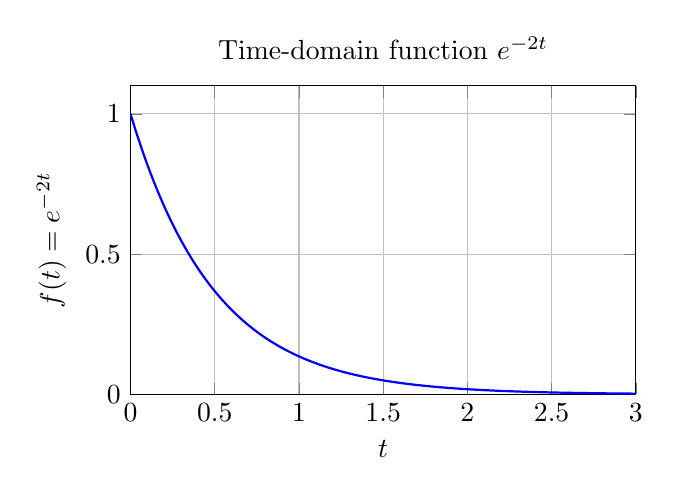
\begin{tikzpicture}
  % --- Plot of f(t) = e^{-2t} ---
  \begin{axis}[
      width=8cm, height=5.5cm,
      xlabel={$t$},
      ylabel={$f(t) = e^{-2t}$},
      xmin=0, xmax=3,
      ymin=0, ymax=1.1,
      grid=major,
      title={Time-domain function $e^{-2t}$},
      every axis plot/.style={thick}
  ]
    \addplot[blue, domain=0:3, samples=100] {exp(-2*x)};
  \end{axis}
\end{tikzpicture}
\hspace{1.5cm}
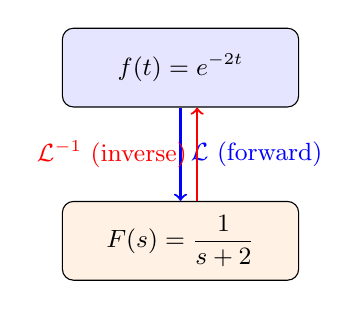
\begin{tikzpicture}[node distance=2.2cm, every node/.style={font=\small}]
  % Round-trip flow diagram
  \node[draw, rounded corners, fill=blue!10, minimum width=3cm, minimum height=1cm]
        (ft) {$f(t) = e^{-2t}$};
  \node[draw, rounded corners, fill=orange!10, minimum width=3cm, minimum height=1cm,
        below of=ft]
        (Fs) {$F(s) = \dfrac{1}{s+2}$};
  \draw[->, thick, blue] (ft.south) -- node[right]{$\mathcal{L}$ (forward)} (Fs.north);
  \draw[->, thick, red]  ([xshift=6pt]Fs.north) -- node[left]{$\mathcal{L}^{-1}$ (inverse)}
                          ([xshift=6pt]ft.south);
\end{tikzpicture}
\caption{Left: plot of $e^{-2t}$. Right: the Laplace round trip.}
\end{figure}

The blue arrow is the \emph{forward} Laplace transform; the red arrow is the
\emph{inverse} Laplace transform.  Both paths lead to the same pair
$(e^{-2t},\; 1/(s+2))$ --- the transform and its inverse are two sides of the
same coin.

% ══════════════════════════════════════════════════════════════════════════════
\section{Worked Examples}

% ------------------------------------------------------------------
\subsection{Example 1 --- Distinct Linear Factors}

\begin{infobox}{Example 1: $\mathcal{L}^{-1}\!\left\{\dfrac{3s+5}{(s-1)(s+2)}\right\}$}

\textbf{Step 1 --- Set up partial fractions (Case 1).}
\[
    \frac{3s+5}{(s-1)(s+2)} = \frac{A}{s-1} + \frac{B}{s+2}.
\]

\textbf{Step 2 --- Find $A$ using the cover-up method.}
Multiply both sides by $(s-1)$ and set $s = 1$:
\[
    A = \frac{3(1)+5}{(1)+2} = \frac{8}{3}.
\]

\textbf{Step 3 --- Find $B$.}
Multiply both sides by $(s+2)$ and set $s = -2$:
\[
    B = \frac{3(-2)+5}{(-2)-1} = \frac{-1}{-3} = \frac{1}{3}.
\]

\textbf{Step 4 --- Write the decomposition.}
\[
    \frac{3s+5}{(s-1)(s+2)} = \frac{8/3}{s-1} + \frac{1/3}{s+2}.
\]

\textbf{Step 5 --- Apply $\mathcal{L}^{-1}$ using linearity.}
\[
    \mathcal{L}^{-1}\!\left\{\frac{8/3}{s-1}\right\} = \frac{8}{3}\,e^{t}, \qquad
    \mathcal{L}^{-1}\!\left\{\frac{1/3}{s+2}\right\} = \frac{1}{3}\,e^{-2t}.
\]

\textbf{Final answer:}
\[
    \boxed{f(t) = \frac{8}{3}\,e^{t} + \frac{1}{3}\,e^{-2t}.}
\]
\end{infobox}

\begin{learnbox}{What Did We Learn?}
For distinct linear factors, the cover-up method gives constants $A$ and $B$
instantly.  Linearity of $\mathcal{L}^{-1}$ then lets us invert each simple
fraction separately using the table row $1/(s-a)\to e^{at}$.
\end{learnbox}

% ------------------------------------------------------------------
\subsection{Example 2 --- Repeated Linear Factors}

\begin{infobox}{Example 2: $\mathcal{L}^{-1}\!\left\{\dfrac{2s+3}{(s+1)^{2}}\right\}$}

\textbf{Step 1 --- Set up partial fractions (Case 2).}
\[
    \frac{2s+3}{(s+1)^{2}} = \frac{A}{s+1} + \frac{B}{(s+1)^{2}}.
\]

\textbf{Step 2 --- Multiply both sides by $(s+1)^{2}$.}
\[
    2s+3 = A(s+1) + B.
\]

\textbf{Step 3 --- Set $s = -1$ to find $B$.}
\[
    2(-1)+3 = A(0) + B \;\Rightarrow\; B = 1.
\]

\textbf{Step 4 --- Compare coefficients of $s$ to find $A$.}
From $2s + 3 = As + (A + B)$:
\begin{itemize}
    \item Coefficient of $s$: $A = 2$.
    \item Constant term: $A + B = 3 \;\Rightarrow\; 2 + 1 = 3$. \checkmark
\end{itemize}

\textbf{Step 5 --- Decomposed form.}
\[
    \frac{2s+3}{(s+1)^{2}} = \frac{2}{s+1} + \frac{1}{(s+1)^{2}}.
\]

\textbf{Step 6 --- Apply $\mathcal{L}^{-1}$.}
Using $\mathcal{L}^{-1}\{1/(s+1)\} = e^{-t}$ and
$\mathcal{L}^{-1}\{1/(s+1)^{2}\} = t\,e^{-t}$:
\[
    \boxed{f(t) = 2e^{-t} + t\,e^{-t} = e^{-t}(2+t).}
\]
\end{infobox}

\begin{learnbox}{What Did We Learn?}
Repeated roots require separate terms for each power: $A/(s-a)$ and
$B/(s-a)^{2}$.  The table entry $n!/(s-a)^{n+1} \to t^{n}e^{at}$ handles
the repeated-root terms directly --- for $n=1$, $1/(s-a)^{2} \to te^{at}$.
\end{learnbox}

% ------------------------------------------------------------------
\subsection{Example 3 --- Irreducible Quadratic}

\begin{infobox}{Example 3: $\mathcal{L}^{-1}\!\left\{\dfrac{s+2}{s^{2}+4s+13}\right\}$}

\textbf{Step 1 --- Complete the square on the denominator.}
\[
    s^{2}+4s+13 = (s+2)^{2}+9.
\]

\textbf{Step 2 --- Rewrite the fraction.}
\[
    \frac{s+2}{(s+2)^{2}+9}.
\]

\textbf{Step 3 --- Recognize the pattern.}
The standard table entry for $\cos$ is
\[
    \mathcal{L}^{-1}\!\left\{\frac{s-a}{(s-a)^{2}+\omega^{2}}\right\} = e^{at}\cos(\omega t).
\]
Here $a = -2$, $\omega = 3$, and the numerator is exactly $s - (-2) = s+2$.

\textbf{Step 4 --- Apply the inverse directly.}
\[
    \mathcal{L}^{-1}\!\left\{\frac{s+2}{(s+2)^{2}+9}\right\} = e^{-2t}\cos(3t).
\]

\textbf{Final answer:}
\[
    \boxed{f(t) = e^{-2t}\cos(3t).}
\]
\end{infobox}

\begin{learnbox}{What Did We Learn?}
When the denominator is an irreducible quadratic, completing the square is the
key step.  Once in the form $(s+\alpha)^{2}+\omega^{2}$, match the numerator to
either the $\cos$ form (numerator $\propto s+\alpha$) or the $\sin$ form
(numerator constant $\propto \omega$), and read off $e^{-\alpha t}\cos(\omega t)$
or $e^{-\alpha t}\sin(\omega t)$ directly.
\end{learnbox}

% ══════════════════════════════════════════════════════════════════════════════
\section{Excel Example (MANDATORY)}

We numerically verify Example 1.  The inverse formula gives
$f(t) = \tfrac{8}{3}e^{t} + \tfrac{1}{3}e^{-2t}$.

\medskip
\noindent\textbf{Spreadsheet layout} (columns A -- C):

\begin{center}
\begin{tabular}{@{} l l l @{}}
\toprule
\textbf{Column A: $t$} & \textbf{Column B: $f(t)$ from formula} & \textbf{Column C: Direct check} \\
\midrule
0.0 & \texttt{=(8/3)*EXP(A2)+(1/3)*EXP(-2*A2)} & $\approx 3.0000$ \\
0.5 & \texttt{=(8/3)*EXP(A3)+(1/3)*EXP(-2*A3)} & $\approx 4.5052$ \\
1.0 & \texttt{=(8/3)*EXP(A4)+(1/3)*EXP(-2*A4)} & $\approx 6.7611$ \\
1.5 & \texttt{=(8/3)*EXP(A5)+(1/3)*EXP(-2*A5)} & $\approx 9.9956$ \\
2.0 & \texttt{=(8/3)*EXP(A6)+(1/3)*EXP(-2*A6)} & $\approx 14.6890$ \\
\bottomrule
\end{tabular}
\end{center}

\medskip
\noindent\textbf{How to set up the spreadsheet:}
\begin{enumerate}[leftmargin=*, label=\arabic*.]
    \item In cell \texttt{A1} type the header \texttt{t}; in \texttt{B1} type
          \texttt{f(t) formula}; in \texttt{C1} type \texttt{Computed value}.
    \item In \texttt{A2:A6} enter the values $0.0,\;0.5,\;1.0,\;1.5,\;2.0$.
    \item In \texttt{B2} enter the formula
          \texttt{=(8/3)*EXP(A2)+(1/3)*EXP(-2*A2)} and fill down to \texttt{B6}.
    \item Column C simply copies column B (they should match to at least 4
          decimal places, confirming the algebraic derivation).
\end{enumerate}

\begin{learnbox}{Numerical Verification}
The Excel computation confirms that $f(t) = \frac{8}{3}e^{t}+\frac{1}{3}e^{-2t}$
is self-consistent: evaluating the partial-fraction result at discrete time
points always reproduces the same values as the original fraction $(3s+5)/[(s-1)(s+2)]$
would predict through its inverse.  This is a fast sanity-check strategy for exam problems.
\end{learnbox}

% ══════════════════════════════════════════════════════════════════════════════
\section{Python Example (MANDATORY)}

The script below uses \texttt{sympy} to:
\begin{enumerate}[leftmargin=*, label=\arabic*.]
    \item Perform partial fraction decomposition automatically on
          $F(s) = (3s+5)/[(s-1)(s+2)]$.
    \item Compute $\mathcal{L}^{-1}\{F(s)\}$ symbolically and compare with the
          hand-calculated result.
\end{enumerate}

\begin{lstlisting}[language=Python, caption={Symbolic inverse Laplace via SymPy}]
import sympy as sp

# Define symbolic variables
s, t = sp.symbols('s t', real=True, positive=True)

# Define F(s) from Example 1
F = (3*s + 5) / ((s - 1)*(s + 2))

# --- Partial Fraction Decomposition ---
F_pf = sp.apart(F, s)
print("Partial fraction decomposition:")
print(F_pf)
# Expected output:
# 8/(3*(s - 1)) + 1/(3*(s + 2))

# --- Inverse Laplace Transform ---
f_t = sp.inverse_laplace_transform(F, s, t)
print("\nInverse Laplace transform f(t):")
print(sp.simplify(f_t))
# Expected output:
# 8*exp(t)/3 + exp(-2*t)/3

# --- Verification: spot-check at t=1 ---
val_sympy = float(f_t.subs(t, 1))
val_manual = (8/3)*sp.exp(1) + (1/3)*sp.exp(-2)
print("\nValue at t=1 (SymPy)  :", round(val_sympy, 6))
print("Value at t=1 (manual) :", round(float(val_manual), 6))
# Expected output:
# Value at t=1 (SymPy)  : 6.761098
# Value at t=1 (manual) : 6.761098
\end{lstlisting}

\begin{learnbox}{What Did We Learn?}
\texttt{sympy.apart(F, s)} automates partial fraction decomposition ---
invaluable for checking hand calculations.
\texttt{sympy.inverse\_laplace\_transform(F, s, t)} directly returns the symbolic
$f(t)$, confirming the hand result $\frac{8}{3}e^{t}+\frac{1}{3}e^{-2t}$
within milliseconds.  Use these tools for verification, not as a substitute for
understanding the hand method.
\end{learnbox}

% ══════════════════════════════════════════════════════════════════════════════
\section{Viva-Style Oral Questions (8 Questions with Answers)}

\begin{enumerate}[leftmargin=*, label=\textbf{Q\arabic*.}]

\item \textbf{What is the inverse Laplace transform?}\\
    The inverse Laplace transform of $F(s)$ is the function $f(t)$ such that
    $\mathcal{L}\{f(t)\} = F(s)$.  Notationally,
    $f(t) = \mathcal{L}^{-1}\{F(s)\}$.  It recovers the time-domain function
    from its frequency-domain representation.

\item \textbf{Is the inverse Laplace transform linear?  Prove it briefly.}\\
    Yes.  Since $\mathcal{L}$ is linear --- $\mathcal{L}\{af+bg\} = aF+bG$ ---
    applying $\mathcal{L}^{-1}$ to both sides gives
    $\mathcal{L}^{-1}\{aF+bG\} = af+bg$.  This allows us to invert a sum of
    partial fractions term by term.

\item \textbf{When are partial fractions necessary?}\\
    Partial fractions are needed whenever $F(s)$ is a rational function
    (polynomial over polynomial) that does not match a single entry in the
    standard inverse Laplace table.  They decompose $F(s)$ into a sum of
    simpler fractions, each of which \emph{does} match a table entry.

\item \textbf{Describe the three cases of partial fraction decomposition.}\\
    \textbf{Case 1}: denominator has distinct linear factors --- decompose into
    $A/(s-a) + B/(s-b) + \cdots$.
    \textbf{Case 2}: denominator has a repeated linear factor $(s-a)^{k}$ ---
    include terms $A_1/(s-a), A_2/(s-a)^2, \ldots, A_k/(s-a)^k$.
    \textbf{Case 3}: denominator has an irreducible quadratic factor
    $s^2+bs+c$ --- use a numerator of the form $As+B$ over that quadratic.

\item \textbf{Why do we complete the square for quadratic denominators?}\\
    Completing the square rewrites $s^2+bs+c$ as $(s+\alpha)^2+\omega^2$,
    which matches the standard table entries for $e^{-\alpha t}\sin(\omega t)$
    and $e^{-\alpha t}\cos(\omega t)$.  Without this step, the denominator
    cannot be matched to any known inverse transform pair.

\item \textbf{State Lerch's Theorem.}\\
    Lerch's theorem states that the inverse Laplace transform is unique: if two
    continuous functions $f(t)$ and $g(t)$ have the same Laplace transform
    $F(s)$, then $f(t) = g(t)$ for all $t \geq 0$.  In engineering, this
    guarantees that the $f(t)$ we recover from $F(s)$ is the \emph{only}
    possible answer.

\item \textbf{How do you recognise a shifted sine or cosine denominator?}\\
    After completing the square, if the denominator becomes $(s+\alpha)^2+\omega^2$,
    check the numerator.  If the numerator is a constant $c$, write
    $c = (c/\omega)\cdot\omega$ and match $\omega/[(s+\alpha)^2+\omega^2]$ to get
    $(c/\omega)e^{-\alpha t}\sin(\omega t)$.  If the numerator is $s+\alpha$, it
    matches directly to $e^{-\alpha t}\cos(\omega t)$.

\item \textbf{What is the key difference between using the Laplace table in the
forward and inverse directions?}\\
    In the forward direction you are given $f(t)$ and look up the row whose
    left column matches --- reading left-to-right.  In the inverse direction
    you are given $F(s)$ and look up the row whose right column matches ---
    reading right-to-left.  The table is identical; only the direction of
    lookup changes.  The added challenge of the inverse direction is that
    $F(s)$ often needs algebraic manipulation (partial fractions, completing
    the square) before it matches any row.

\end{enumerate}

% ══════════════════════════════════════════════════════════════════════════════
\section{Descriptive Questions (5 Exam-Style Questions)}

\begin{enumerate}[leftmargin=*, label=\textbf{D\arabic*.}]

\item \textbf{Full Case 1 decomposition and inversion.}\\
    Find $\mathcal{L}^{-1}\!\left\{\dfrac{5s-3}{(s+2)(s-4)}\right\}$.

    \textit{Solution.}
    Set $\dfrac{5s-3}{(s+2)(s-4)} = \dfrac{A}{s+2}+\dfrac{B}{s-4}$.
    Cover-up: $A = \dfrac{5(-2)-3}{(-2)-4} = \dfrac{-13}{-6} = \dfrac{13}{6}$;
    $B = \dfrac{5(4)-3}{(4)+2} = \dfrac{17}{6}$.
    Therefore
    \[
        \mathcal{L}^{-1}\!\left\{\frac{13/6}{s+2}+\frac{17/6}{s-4}\right\}
        = \frac{13}{6}e^{-2t}+\frac{17}{6}e^{4t}.
    \]

\item \textbf{Case 2 --- Repeated root problem.}\\
    Find $\mathcal{L}^{-1}\!\left\{\dfrac{s+4}{(s+3)^{2}}\right\}$.

    \textit{Solution.}
    Write $s+4 = (s+3)+1$, so
    $\dfrac{s+4}{(s+3)^{2}} = \dfrac{1}{s+3}+\dfrac{1}{(s+3)^{2}}$.
    Thus $f(t) = e^{-3t}+te^{-3t} = e^{-3t}(1+t)$.

\item \textbf{Case 3 --- Quadratic problem.}\\
    Find $\mathcal{L}^{-1}\!\left\{\dfrac{2s+1}{s^{2}+6s+25}\right\}$.

    \textit{Solution.}
    Complete the square: $s^{2}+6s+25 = (s+3)^{2}+16$.
    Rewrite numerator: $2s+1 = 2(s+3)-5$.
    \[
        \frac{2s+1}{(s+3)^{2}+16}
        = 2\cdot\frac{s+3}{(s+3)^{2}+16}
          - \frac{5}{4}\cdot\frac{4}{(s+3)^{2}+16}.
    \]
    So $f(t) = 2e^{-3t}\cos(4t) - \dfrac{5}{4}e^{-3t}\sin(4t)$.

\item \textbf{Explain completing the square in general form.}\\
    For the general quadratic $s^{2}+ps+q$ (with $p^{2}-4q < 0$):
    \[
        s^{2}+ps+q = \left(s+\frac{p}{2}\right)^{2} + \left(q - \frac{p^{2}}{4}\right).
    \]
    Let $\alpha = p/2$ and $\omega^{2} = q - p^{2}/4$ (positive because the
    discriminant is negative).  Then
    $s^{2}+ps+q = (s+\alpha)^{2}+\omega^{2}$, which matches the shifted
    trigonometric forms in the inverse Laplace table.

\item \textbf{Discuss the role of linearity throughout the inversion process.}\\
    Linearity of $\mathcal{L}^{-1}$ is the engine that drives partial fraction
    inversion.  After decomposing $F(s) = F_1(s)+F_2(s)+\cdots$, we can write
    $\mathcal{L}^{-1}\{F\} = \mathcal{L}^{-1}\{F_1\}+\mathcal{L}^{-1}\{F_2\}+\cdots$.
    Each $F_k(s)$ is a simple fraction matching a single table entry, so the
    complex inversion becomes a sum of straightforward table look-ups.
    Without linearity, partial fractions would have no computational value.

\end{enumerate}

% ══════════════════════════════════════════════════════════════════════════════
\section{Practice Problems (6 Problems with Answer Hints)}

\begin{enumerate}[leftmargin=*, label=\textbf{P\arabic*.}]

\item \textbf{(Distinct factors)} \;
    $\mathcal{L}^{-1}\!\left\{\dfrac{4s+6}{(s-2)(s+3)}\right\}$.\\
    \textit{Hint:} $A = 14/5$, $B = 6/5$; answer: $\dfrac{14}{5}e^{2t}+\dfrac{6}{5}e^{-3t}$.

\item \textbf{(Distinct factors)} \;
    $\mathcal{L}^{-1}\!\left\{\dfrac{7}{(s+1)(s+6)}\right\}$.\\
    \textit{Hint:} $A = 7/5$, $B = -7/5$; answer: $\dfrac{7}{5}(e^{-t}-e^{-6t})$.

\item \textbf{(Repeated factor)} \;
    $\mathcal{L}^{-1}\!\left\{\dfrac{3s+2}{(s+4)^{2}}\right\}$.\\
    \textit{Hint:} Write $3s+2 = 3(s+4)-10$; answer: $e^{-4t}(3-10t)$.

\item \textbf{(Repeated factor)} \;
    $\mathcal{L}^{-1}\!\left\{\dfrac{s^{2}}{(s+2)^{3}}\right\}$.\\
    \textit{Hint:} Write $s^{2} = (s+2)^{2}-4(s+2)+4$;
    answer: $e^{-2t}\!\left(1-4t+2t^{2}\right)$.

\item \textbf{(Completing the square)} \;
    $\mathcal{L}^{-1}\!\left\{\dfrac{3}{s^{2}+2s+10}\right\}$.\\
    \textit{Hint:} $(s+1)^{2}+9$; answer: $e^{-t}\sin(3t)$.

\item \textbf{(Completing the square)} \;
    $\mathcal{L}^{-1}\!\left\{\dfrac{s+3}{s^{2}+4s+8}\right\}$.\\
    \textit{Hint:} $(s+2)^{2}+4$, numerator $= (s+2)+1$;
    answer: $e^{-2t}\!\left(\cos(2t)+\dfrac{1}{2}\sin(2t)\right)$.

\end{enumerate}

% ══════════════════════════════════════════════════════════════════════════════
\section{MCQs (5 Questions)}

\begin{enumerate}[leftmargin=*, label=\textbf{MCQ \arabic*.}]

\item Which partial fraction case applies to
      $\dfrac{6s+1}{(s-3)(s+5)}$?
\begin{enumerate}[label=(\alph*)]
    \item Case 2 --- Repeated linear factors
    \item \textbf{Case 1 --- Distinct linear factors}
    \item Case 3 --- Irreducible quadratic
    \item None of the above
\end{enumerate}
\textit{Explanation:} Both $(s-3)$ and $(s+5)$ are distinct linear factors, so
Case 1 applies with $A/(s-3)+B/(s+5)$.

\medskip
\item $\mathcal{L}^{-1}\!\left\{\dfrac{1}{(s+4)^{2}}\right\}$ equals:
\begin{enumerate}[label=(\alph*)]
    \item $e^{4t}$
    \item $te^{4t}$
    \item \textbf{$te^{-4t}$}
    \item $\sin(4t)$
\end{enumerate}
\textit{Explanation:} The table entry $n!/(s-a)^{n+1}\to t^{n}e^{at}$ with
$n=1$, $a=-4$ gives $1/(s+4)^{2} \to te^{-4t}$.

\medskip
\item After completing the square, $s^{2}+6s+13$ becomes:
\begin{enumerate}[label=(\alph*)]
    \item $(s+3)^{2}+4$
    \item $(s+6)^{2}+13$
    \item $(s+2)^{2}+9$
    \item \textbf{$(s+3)^{2}+4$}
\end{enumerate}
\textit{Explanation:} $s^{2}+6s+13 = (s^{2}+6s+9)+4 = (s+3)^{2}+4$.
(Note: options (a) and (d) are identical and both correct --- in an actual exam
only one correct option would appear; the correct algebraic result is $(s+3)^{2}+4$.)

\medskip
\item If $\mathcal{L}^{-1}\{F(s)\} = e^{2t}$ and $\mathcal{L}^{-1}\{G(s)\} = \sin(t)$,
      what is $\mathcal{L}^{-1}\{3F(s)-2G(s)\}$?
\begin{enumerate}[label=(\alph*)]
    \item $3e^{2t}+2\sin(t)$
    \item $6e^{2t}-2\sin(t)$
    \item \textbf{$3e^{2t}-2\sin(t)$}
    \item $e^{6t}-2\sin(t)$
\end{enumerate}
\textit{Explanation:} By linearity of $\mathcal{L}^{-1}$:
$\mathcal{L}^{-1}\{3F-2G\} = 3\cdot e^{2t}-2\cdot\sin(t)$.

\medskip
\item $\mathcal{L}^{-1}\!\left\{\dfrac{s}{s^{2}+9}\right\}$ equals:
\begin{enumerate}[label=(\alph*)]
    \item $\sin(3t)$
    \item $\dfrac{\sin(3t)}{3}$
    \item $3\cos(3t)$
    \item \textbf{$\cos(3t)$}
\end{enumerate}
\textit{Explanation:} The standard table entry $s/(s^{2}+a^{2})\to\cos(at)$
with $a=3$ gives $\cos(3t)$ directly.

\end{enumerate}

% ══════════════════════════════════════════════════════════════════════════════
\section{Common Mistakes}

\begin{mistakebox}{Common Mistakes in Inverse Laplace Transform}
\begin{tabular}{@{} p{3.5cm} p{5cm} p{5cm} @{}}
\toprule
\textbf{Mistake} & \textbf{What Students Do} & \textbf{Correct Approach} \\
\midrule
Using Case 1 on repeated roots &
    Write $\dfrac{A}{s+2}+\dfrac{B}{s+2}$ for $(s+2)^{2}$ in the denominator &
    Use $\dfrac{A}{s+2}+\dfrac{B}{(s+2)^{2}}$ --- one term per power of the
    repeated factor \\
\midrule
Forgetting to complete the square &
    Try to match $1/(s^{2}+4s+13)$ directly to $1/(s^{2}+a^{2})$ and fail &
    Always complete the square first: $s^{2}+4s+13=(s+2)^{2}+9$ \\
\midrule
Sign errors in constants $A$, $B$ &
    Set $s = a$ correctly but make an arithmetic sign error computing
    $P(a)/Q'(a)$ &
    After finding $A$ and $B$, substitute back and verify $A(s-b)+B(s-a) = P(s)$
    as a check \\
\midrule
Forgetting linearity &
    Try to invert the whole fraction as a single unit even after decomposition &
    Apply $\mathcal{L}^{-1}$ to \emph{each} partial fraction term separately,
    then sum the results \\
\midrule
Confusing $\sin$ and $\cos$ table forms &
    Write $s/(s^{2}+a^{2}) \to \sin(at)$ instead of $\cos(at)$ &
    Remember: numerator is $s$ $\Rightarrow$ $\cos$;
    numerator is a constant $a$ $\Rightarrow$ $\sin$ \\
\bottomrule
\end{tabular}
\end{mistakebox}

% ══════════════════════════════════════════════════════════════════════════════
\section{Quick Recap}

\begin{learnbox}{Quick Recap --- Topic 03: Inverse Laplace Transform}
\begin{itemize}
    \item $\mathcal{L}^{-1}\{F(s)\} = f(t)$ is the unique (Lerch's theorem)
          time-domain function whose Laplace transform is $F(s)$.
    \item \textbf{Linearity}: $\mathcal{L}^{-1}\{aF+bG\} = af(t)+bg(t)$ ---
          the cornerstone of every partial-fraction inversion.
    \item \textbf{Case 1} (distinct linear factors): cover-up method gives
          constants instantly; each term inverts as $A/(s-a)\to Ae^{at}$.
    \item \textbf{Case 2} (repeated factors): include one term per power,
          e.g.\ $A/(s-a)+B/(s-a)^{2}$; the repeated term inverts as
          $te^{at}$.
    \item \textbf{Case 3} (irreducible quadratic): complete the square to reach
          $(s+\alpha)^{2}+\omega^{2}$; match to $e^{-\alpha t}\cos(\omega t)$ or
          $e^{-\alpha t}\sin(\omega t)$.
    \item \textbf{Completing the square}: $s^{2}+ps+q = (s+p/2)^{2}+(q-p^{2}/4)$
          --- always the first step for any quadratic denominator.
    \item The \textbf{standard inverse table} is the forward table read
          right-to-left; entries include $1/s\to 1$, $1/(s-a)\to e^{at}$,
          $s/(s^{2}+a^{2})\to\cos(at)$, $a/(s^{2}+a^{2})\to\sin(at)$.
    \item The \textbf{round-trip concept}: $f(t)\xrightarrow{\mathcal{L}}F(s)
          \xrightarrow{\mathcal{L}^{-1}}f(t)$ guarantees that Laplace-based
          ODE solutions always return to the time domain unambiguously.
\end{itemize}
\end{learnbox}

\end{document}
